% ***********************************
% *** Bext to compile with xetex  ***
% *** Requires UTF-8 file format! ***
% ***********************************
% 
% - Author: Aleksander Sandro GRM
% - Date: 21/08/2023
%
%
% ***************************
% *** Beamer frame format ***
% ***************************
%
\documentclass[8pt,aspectratio=169]{beamer} % 16:9

%
% - additional formats are: 169, 1610, 149, 54, 43 and 32
%
%\documentclass[8pt,aspectratio=43]{beamer} % (old format 4:3)

%
% *** UTF-8 coding ***
%
% Comment if compiled with xelatex, unless uncomment for pdflatex!
%
%\usepackage[utf8x]{inputenc} % needed for pdflatex

%
% *** Language setup ***
%
\usepackage[slovene]{babel}
%\usepackage[english]{babel}


% 
% *** coloring hyper references  ***
%
%  In class Beamer \usepackage{hyperref} already loaded
%
\hypersetup{
	colorlinks = true,
	linkcolor = {red!50!black},
	citecolor = {blue!50!black},
	urlcolor = {blue!90!black}
}


%
% *** Beamer ***
%
\usepackage{etex}
\usepackage{wasysym}
\usepackage{animate}
\usepackage{xmpmulti}

%
% *** New Theme Definitions ***
%

%\useoutertheme[subsection=false]{smoothbars}
\definecolor{royalblue1}{RGB}{72,118,255}
\definecolor{shadowbg}{RGB}{51,51,51}
\definecolor{titlebg}{RGB}{51,51,51}
\definecolor{royalblue4}{RGB}{39,64,139}
\definecolor{navyblue}{RGB}{0, 0, 127}
\definecolor{deepcarminepink}{rgb}{0.94, 0.19, 0.22}

\usetheme{Warsaw}
\usecolortheme[RGB={72,118,255}]{structure} 
\usetheme[height=7mm]{Rochester} 
\setbeamertemplate{items}[ball] 
\setbeamertemplate{blocks}[rounded][shadow=true] 
\usefonttheme[onlymath]{serif}
%
\setbeamercolor{normal text}{fg=navyblue,bg=white}
\setbeamercolor{secsubsec}{fg=white,bg=royalblue1}
\setbeamercolor{shadow}{fg=secinhead,bg=shadowbg}
\setbeamercolor{frametitle}{fg=white,bg=royalblue4}
\setbeamercolor{math text}{fg=black}

%
% *** Page setup ***
%
\setbeamersize{text margin  left=1cm} % <- like this
\setbeamersize{text margin right=1cm} % <- like this
\usepackage{ragged2e}
\justifying

%
% *** include packages ***
%
\usepackage{graphicx}
\usepackage{xcolor}
\usepackage{subfigure}
\usepackage{multicol}
\usepackage{mathtools}
\usepackage{amsmath,amsthm,amssymb,latexsym}
\usepackage{empheq}
\usepackage[many]{tcolorbox}
\usepackage{siunitx}
\usepackage{dirtree}
%
\usepackage[all,knot]{xy}
\xyoption{arc}
\usepackage{url}
\usepackage{multimedia}
\usepackage{setspace}
\usepackage{textcomp}
\usepackage{bm}
\usepackage{xfrac}
\usepackage{tikz}
\usepackage{cancel}
\usetikzlibrary{shadings}
\usepackage{tikzsymbols}

\setbeamertemplate{headline}
{
	\leavevmode%
	\hbox{%
		\begin{beamercolorbox}[wd=\paperwidth,ht=2.5ex,dp=1ex]{secsubsec}%
			\raggedright
			\hspace*{2em}%
			{\bfseries\sffamily\tiny\color{white}~\insertsection\hfill\insertsubsection}%
			%\thesection.~\insertsection\hfill\insertsubsection}%
			\hspace*{2em}%
		\end{beamercolorbox}%
	}
	%\vskip-1pt%
	\hbox{%
		%\tikz\draw[draw=none,top color=royalblue1,bottom color=royalblue4!60] (0,0) rectangle (\paperwidth,0.1);
		\tikz\draw[draw=none,top color=black,bottom color=black] (0,0) rectangle (\paperwidth,0.05);
	}%
}

\setbeamertemplate{frametitle}
{\vskip-2.5pt
	\leavevmode
	\hbox{%
		\begin{beamercolorbox}[wd=\paperwidth,ht=1.8ex,dp=1ex]{frametitle}%
			\raggedright\hspace*{2em}\small\insertframetitle
		\end{beamercolorbox}
	}%
}

% clean navigation
\setbeamertemplate{navigation symbols}{}{}

% add frame number
\newcommand*\oldmacro{}%
\let\oldmacro\insertshorttitle%
\renewcommand*\insertshorttitle{%
	\oldmacro\hfill%
	\insertframenumber\,/\,\inserttotalframenumber%
}


% ****************************
% *** Numbered environment ***
% ****************************
\newenvironment{primer}[1][]{\noindent \textbf{Primer} }{\medskip}
\newenvironment{sol}[1][]{\noindent \textbf{Rešitev} }{\medskip}


% *********************
% *** notations.tex ***
% *********************
% 
%       *** Latex additions ***
% 
% - Author: aleksander.grm@fpp.uni-lj.si 
% - Date: 02/03/2024 (last modified)

%
% *** Needed packages ***
%
\usepackage{dsfont}

%
% *** New Commands ***
%
%\newcommand*{\point}[1]{\vec{\mkern0mu#1}}
\newcommand{\ci}[0]{\perp\!\!\!\!\!\perp} % conditional independence
\newcommand{\point}[1]{{#1}} % points 
\renewcommand{\vec}[1]{\boldsymbol{#1}}  % math vector
\newcommand{\uvec}[1]{\mathbf{\hat{#1}}} % unit vector
%\newcommand{\mat}[1]{\boldsymbol{#1}}    % matrix
\newcommand{\mat}[1]{\boldsymbol{\mathsf{#1}}}    % matrix
\newcommand{\RR}[0]{\mathbb{R}} % real numbers
\newcommand{\ZZ}[0]{\mathbb{Z}} % integers
\newcommand{\NN}[0]{\mathbb{N}} % natural numbers
\newcommand{\QQ}[0]{\mathbb{Q}} % rational numbers
\newcommand{\CC}[0]{\mathbb{C}} % complex numbers
\newcommand{\tr}[0]{\text{tr}} % trace
\renewcommand{\d}[0]{\mathrm{d}} % total derivative
\newcommand{\prt}[0]{\partial}
\newcommand{\inv}{^{-1}} % inverse
\newcommand{\id}{\mathrm{id}} % identity mapping
\renewcommand{\dim}{\mathrm{dim}} % dimension
%\newcommand{\dim}[1]{\text{\textsc{dim}}\left(#1\right)} 
\newcommand{\adj}[1]{\mathrm{adj}(#1)} % adjoint or adjugate matrix
\newcommand{\rank}[1]{\mathrm{rk}(#1)} % rank
\newcommand{\trace}[1]{\mathrm{sl}(#1)} % trace ali sled
\newcommand{\determ}[1]{\mathrm{det}(#1)} % determinant
%\renewcommand{\det}[1]{\mathrm{det}(#1)} % determinant
\newcommand{\scp}[2]{\langle #1 , #2 \rangle}
\newcommand{\kernel}[1]{\mathrm{ker}({#1})} % kernel/nullspace
\newcommand{\img}[0]{\mathrm{Im}} % image
\newcommand{\idx}[1]{{(#1)}} % index
\newcommand{\diag}[1]{{\mathrm{diag}(#1)}} % diagonal operator
\newcommand{\cov}[1]{{\mathrm{cov}(#1)}} % covariance (matrix) 
\newcommand{\mean}{\mathds{E}} % expectation
\newcommand{\var}{\mathds{V}} % variance
\newcommand{\gauss}[2]{\mathcal{N}\big(#1,\,#2\big)} % gaussian distribution N(.,.)
\newcommand{\gaussx}[3]{\mathcal{N}\big(#1\,|\,#2,\,#3\big)} % gaussian distribution N(.|.,.)
\newcommand{\gaussBig}[2]{\mathcal{N}\left(#1,\,#2\right)} % see above, but with brackets that adjust to the height of the arguments
\newcommand{\gaussxBig}[3]{\mathcal{N}\left(#1\,|\,#2,\,#3\right)} % see above, but with brackets that adjust to the height of the arguments

\newcommand{\T}[0]{^\top} % transpose
\newcommand{\imu}[0]{\mathrm{i}} % complex unit i
\newcommand{\matdet}[1]{\left|\begin{matrix}#1\end{matrix}\right|} % determinant of a matrix
\newcommand{\vecnorm}[1]{\lVert#1\rVert}
\newcommand{\absval}[1]{\left|#1\right|}
\newcommand{\scaprod}[2]{\langle #1, #2 \rangle_0}
\newcommand{\operator}[2]{\operatorname{#1}\left[#2\right]}
\newcommand{\order}[1]{\mathcal{O}(#1)}
\newcommand{\vertat}[2]{\left.#1\:\right|_{#2}}
\newcommand{\longprt}[2]{\frac{\prt #1}{\prt #2}}
\newcommand{\longprtt}[2]{\frac{\prt^2 #1}{\prt #2^2}}


%
% *** Arc notations ***
%
\newcommand{\txtdeg}{\si{\degree}}
\newcommand{\txtmin}{\si{\arcmiute}}
\newcommand{\txtsec}{\si{\arcsecond}}
\newcommand{\arcdeg}[1]{\si{\ang{#1;;}}}
\newcommand{\arcmin}[1]{\si{\ang{;#1;}}}
\newcommand{\arcsec}[1]{\si{\ang{;;#1}}}
\newcommand{\posdm}[2]{\si{\ang{#1;#2;}}}
\newcommand{\posdms}[3]{\si{\ang{#1;#2;#3}}}

%
% *** some shotcuts, bolded symbols, fnacy style, ... ***
%
\newcommand{\mc}{\mathcal}
\newcommand{\mb}{\mathbb}
\newcommand{\ul}{\underline}
\newcommand{\tb}{\textbf}
\newcommand{\bk}{\boldkey}
\newcommand{\bs}{\boldsymbol}
\newcommand{\circled}[1]{\tikz[baseline=(char.base)]{\node[shape=circle,draw,inner sep=1pt] (char) {#1};}}

%
% *** Special keywords
%
\newcommand{\cpp}{\textbf{\texttt{c++}}}
\newcommand{\python}{\textbf{\texttt{python}}}

%
% *** dimension less numbers, and other numbers ***
%
\newcommand{\RE}{\text{\textsl{Re}}}
\newcommand{\MA}{\text{\textsl{Ma}}}
\newcommand{\KN}{\text{\textsl{Kn}}}
%\newcommand{\half}{\sfrac{1}{2}}
\newcommand{\half}{1/2}


%
% *** tabular ***
%
\newcommand{\centercell}[1]{\multicolumn{1}{c}{#1}}
\newcommand{\head}[1]{\centercell{\bfseries#1}}

%
% *** various color definitions ***
%
\definecolor{darkgreen}{rgb}{0,0.6,0}
\definecolor{royalblue1}{RGB}{72,118,255}
\definecolor{shadowbg}{RGB}{51,51,51}
\definecolor{titlebg}{RGB}{51,51,51}
\definecolor{royalblue4}{RGB}{39,64,139}
\definecolor{navyblue}{RGB}{0, 0, 127}
\definecolor{deepcarminepink}{rgb}{0.94, 0.19, 0.22}
\definecolor{navy}{rgb}{0.177,0.349,0.529}
\definecolor{navylight}{rgb}{0.761,0.828,0.894}

%
% *** redefine EMPH types ***
%
\newcommand{\missing}[1]{\textcolor{red}{\textbf{???#1???}}}
\newcommand{\emphc}[1]{\textcolor{blue}{\textbf{#1}}}
\newcommand{\emphcb}[1]{\textcolor{deepcarminepink}{\textbf{#1}}}
\newcommand{\myfig}[1]{\iflanguage{english}{\textbf{Figure}}{\textbf{Slika}} #1}
\newcommand{\myeq}[1]{\iflanguage{english}{\textbf{Eq.}}{\textbf{En.}} (#1)}

%
% *** place a colored box around a character ***
%
\gdef\colchar#1#2{%
	\tikz[baseline]{%
		\node[anchor=base,inner sep=2pt,outer sep=0pt,fill = #2!20] {#1};
	}%
}%

%
% *** Trade names, Copy right... ***
%
% \textsuperscript \textsubscript
\newcommand{\matlab}{\texttt{MatLab}\textsuperscript{\textregistered} }


% ***********************************************
% *** Blocks: block, exampleblock, alertblock ***
% ***********************************************

%
% *** Blocks: block, exampleblock, alertblock ***
%
%\definecolor{shadowbga}{RGB}{51,51,51}
\definecolor{myblue}{rgb}{.9, .9, 1}
\definecolor{lightblue}{rgb}{.9, .9, .5}
%\newcommand*\mybluebox[1]{%
	%	\colorbox{myblue}{\hspace{1em}#1\hspace{1em}}}

\newlength\mytemplen
\newsavebox\mytempbox

\makeatletter
\newcommand\mybluebox{%
	\@ifnextchar[%]
	{\@mybluebox}%
	{\@mybluebox[0pt]}}

\def\@mybluebox[#1]{%
	\@ifnextchar[%]
	{\@@mybluebox[#1]}%
	{\@@mybluebox[#1][0pt]}}

\def\@@mybluebox[#1][#2]#3{
	\sbox\mytempbox{#3}%
	\mytemplen\ht\mytempbox
	\advance\mytemplen #1\relax
	\ht\mytempbox\mytemplen
	\mytemplen\dp\mytempbox
	\advance\mytemplen #2\relax
	\dp\mytempbox\mytemplen
	\colorbox{myblue}{\hspace{1em}\usebox{\mytempbox}\hspace{1em}}}
\makeatother


% *** Example Boxed Equation ***
%

% For a single line equation use: box={\mybluebox[5pt][-2pt]}

% \begin{empheq}[box=\mybluebox]{equation*}
	%   c(t) = c_{in}\left[ 1 - \left(1+ \frac{\Delta \phi}{V_0} \: t
	%   \right)^{-\frac{\phi_{in}}{\Delta \phi}} \right]
	% \end{empheq}
%
% \begin{empheq}[box={\mybluebox[5pt]}]{equation*}
	% 	c_i = \sum_j A_{ij}
	% \end{empheq}
%
% \begin{empheq}[box={\mybluebox[2pt][2pt]}]{equation*}
	%	c_i = \langle\psi|\phi\rangle
	% \end{empheq}


% *********************************************************
% *** Inline code listings: Matlab, Python pretty print ***
% *********************************************************

\usepackage{listings}
\usepackage{xcolor}

\definecolor{codegreen}{rgb}{0,0.6,0}
\definecolor{codegray}{rgb}{0.5,0.5,0.5}
\definecolor{codepurple}{rgb}{0.58,0,0.82}
\definecolor{backcolour}{rgb}{0.95,0.95,0.92}

\lstdefinestyle{mystyle}{
	backgroundcolor=\color{backcolour},   
	commentstyle=\color{codegreen},
	keywordstyle=\color{magenta},
	numberstyle=\tiny\color{codegray},
	stringstyle=\color{codepurple},
	basicstyle=\ttfamily\footnotesize,
	breakatwhitespace=false,         
	breaklines=true,                 
	captionpos=b,                    
	keepspaces=true,                 
	numbers=left,                    
	numbersep=5pt,                  
	showspaces=false,                
	showstringspaces=false,
	showtabs=false,                  
	tabsize=2
}


% *** Example ***
 
% language: Matlab-editor, Matlab-Pyglike, Python, Octave, C, C++,
% look in help doc for additional languages  

%\begin{frame}[fragile]{Title}
%
%  \lstinputlisting[language=Octave,style=mystyle]{BitXorMatrix.m}
%
%\end{frame}


% ******************************
% *** Definicija slo za math ***
% ******************************
\newtheorem{izrek}{Izrek}
\newtheorem{lema}[izrek]{Lema}
\newtheorem{trditev}[izrek]{Trditev}
\newtheorem{posledica}[izrek]{Posledica}
\newtheorem{definicija}[izrek]{Definicija}
\newtheorem{vaja}[izrek]{Vaja}



% ********************
% !!!!! Examples !!!!!
% ********************

% 1. Minpage with top
%
%\begin{minipage}[t]{7cm}
%	\vspace{0pt}
%\end{minipage}
%\hfill
%\begin{minipage}[t]{7cm}
%	\vspace{0pt}
%\end{minipage}
% *********************


% ======================================
% =========== Document start ===========
% ======================================

\title{Class Name, Part 01}
\author[A. GRM]{}

\begin{document}

% ======================
% ===== Title page =====
% ======================

\begin{frame}[plain,noframenumbering,label=titlepage]
	\begin{center}
		
\includegraphics[width=7cm]{figs/logo/head.pdf}\\
		\vspace{5mm}%
		\hspace*{0mm}\rule{120mm}{1mm}\\
		\vspace*{-2mm}%
		\hspace*{0mm}\rule{120mm}{0.5mm}\\
		\vspace*{2.5mm}
		{\Huge \textbf{Ime Predmeta}}\\
		\vspace*{0.5mm}
		\hspace*{0mm}\rule{80mm}{0.5mm}\\
		\vspace{2mm}
		\large{\textbf{\textcolor{red}{Naslov predavanja}}}\\[2mm]
		%\normalsize{\textbf{Ključne besede, če je to poterbno}}\\
		%\vspace*{-1mm}%
		\vspace*{-2mm}%
		\hspace*{0mm}\rule{120mm}{0.5mm}\\
		\vspace*{-1.5mm}%
		\hspace*{0mm}\rule{120mm}{1mm}\\
		\vspace*{5mm}
		%
		\small{\textbf{Aleksander GRM}}\\[1mm]
		\footnotesize{\texttt{ \href{mailto:aleksander.grm@fpp.uni-lj.si}{aleksander.grm@fpp.uni-lj.si}}}\\[4mm]
		\small{\textbf{2022/2023}}
	\end{center}
\end{frame}

% ======================

\begin{frame}[plain,noframenumbering,label=contentpage]
	\begin{center}
		\hspace*{0mm}\rule{130mm}{0.5mm}\\
		\vspace{1.5mm}%
		{\Huge \textbf{Vsebina}}\\
		\vspace{-1mm}%
		\hspace*{0mm}\rule{130mm}{0.5mm}
	\end{center}
	%
	\vspace*{5mm}
	%
	\begin{minipage}[t]{5mm}
		~
	\end{minipage}
	\hfill
	\begin{minipage}[t]{135mm}	
		\normalsize
		\tableofcontents[
		sectionstyle=show,
		subsectionstyle=show/show
		]
	\end{minipage}
	\vfill	
\end{frame}



% =======================
% ===== New Section =====
% =======================

\section{Matrike}
\setcounter{section}{1}

% *** Section Frame ***
\begin{frame}[plain,noframenumbering,label=newsection]
	\vfill
	\begin{center}
		\boxed{\textcolor{royalblue1}{\textbf{Poglavje -- \thesection}}}
		
		\vspace*{5mm}
		\textcolor{royalblue1}{\textbf{\insertsectionhead}}
		%\textcolor{royalblue1}{\textbf{\insertsubsectionhead}}
	\end{center}
	\vfill
\end{frame}

% ===================

\begin{frame}
	\frametitle{Uvod 1}
	
	\emphc{Problem:} Poišči \emph{presečiščno} točko treh ravnin, če je \emph{enačba} ravnine zapisana z enačbo
	
	\[
	\alpha x + \beta y + \gamma z = p.
	\]
	
	\emphc{Primer:} Imamo sistem treh ravnin
	
	\begin{equation} \label{eq:plane_system}
		\begin{split}
		4 x + 2 y + z & = 7\\
		2 x + y - z & = 5\\
		x + 2 y + 2 z & = 3
		\end{split}	
	\end{equation}
	
	kjer je potrebno poiskati skupno točko $T(x,y,z)$.
	
\end{frame}

% *******************

\begin{frame}
	\frametitle{Prikaz delovne površine prosojnice \& največja velikost slike}
	
	%
	% Največja slikovna površina pri 16:9 formatu je:
	%  - širina L = 14.0 cm
	%  - višina H = 7.87 cm
	%
	% kot kaže spodnja slika.
	
	\begin{center}
		% Določanje velikosti slike:
		% - ohranimo "aspect ratio"
		%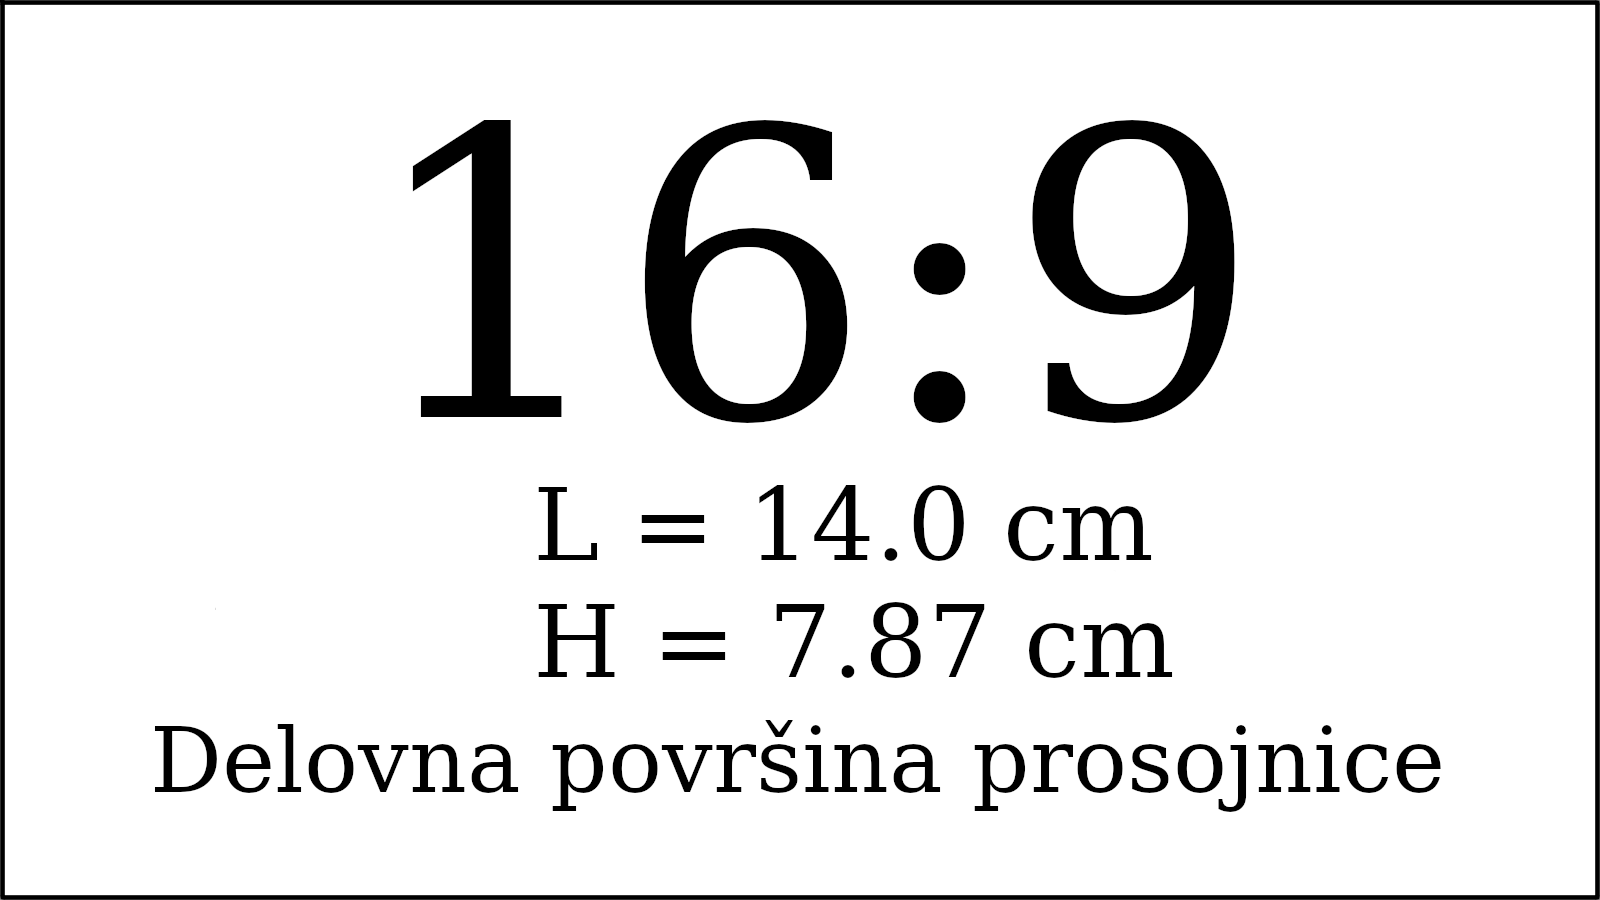
\includegraphics[width=13.9cm]{figs/169_frame.png} % dolžina
		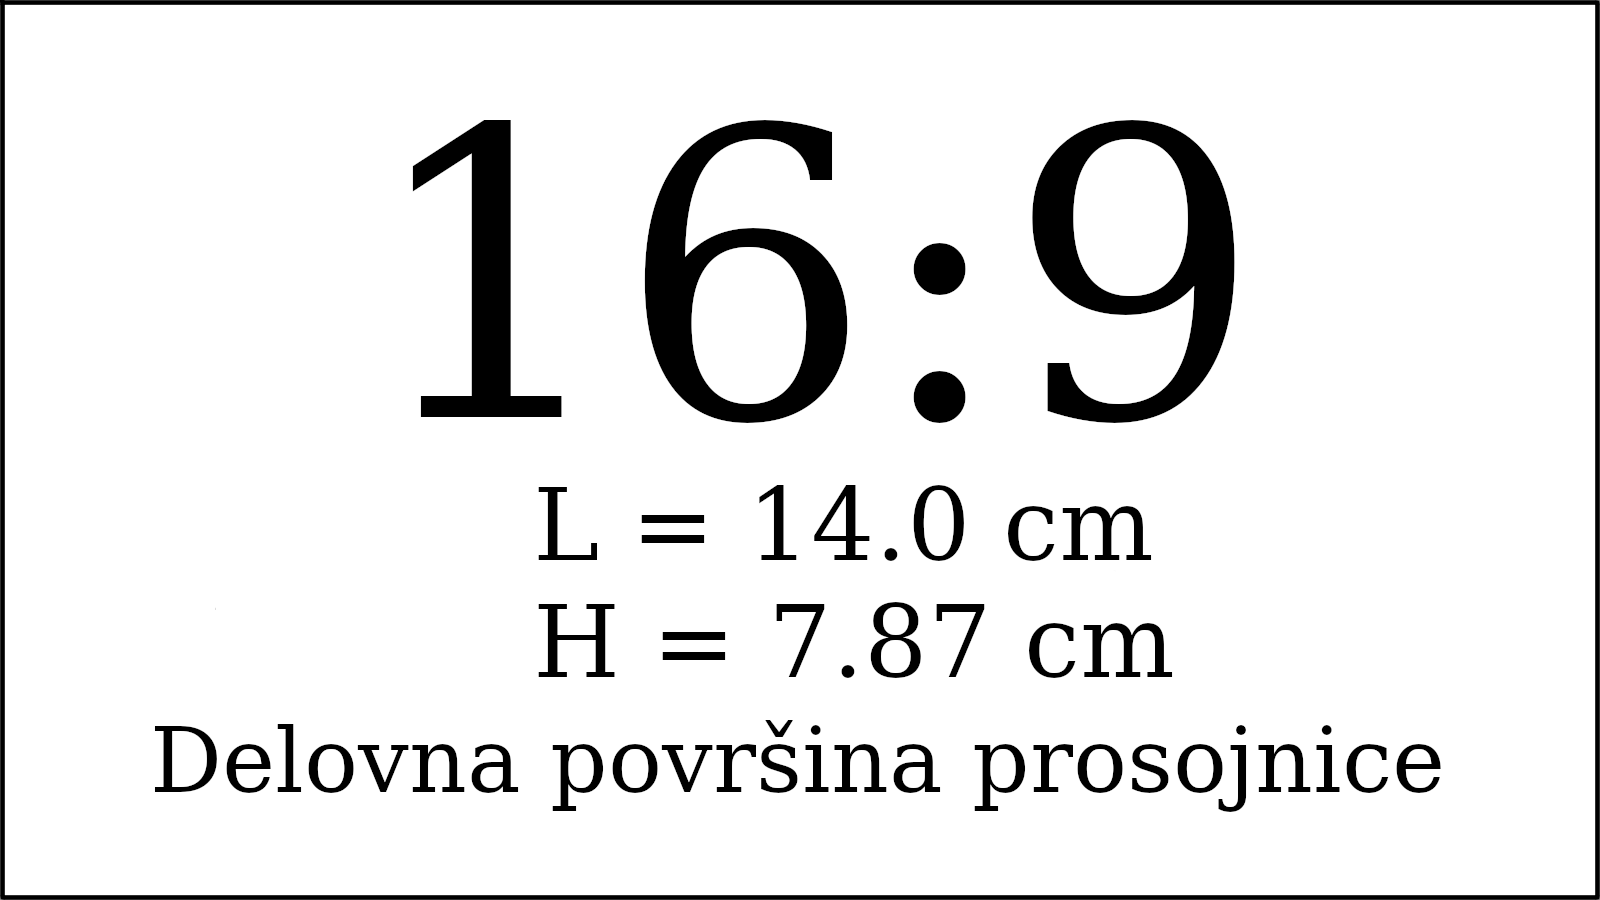
\includegraphics[height=7.7cm]{figs/169_frame.png} % višina
		%
		% - pokvarimo "aspect ratio"
		%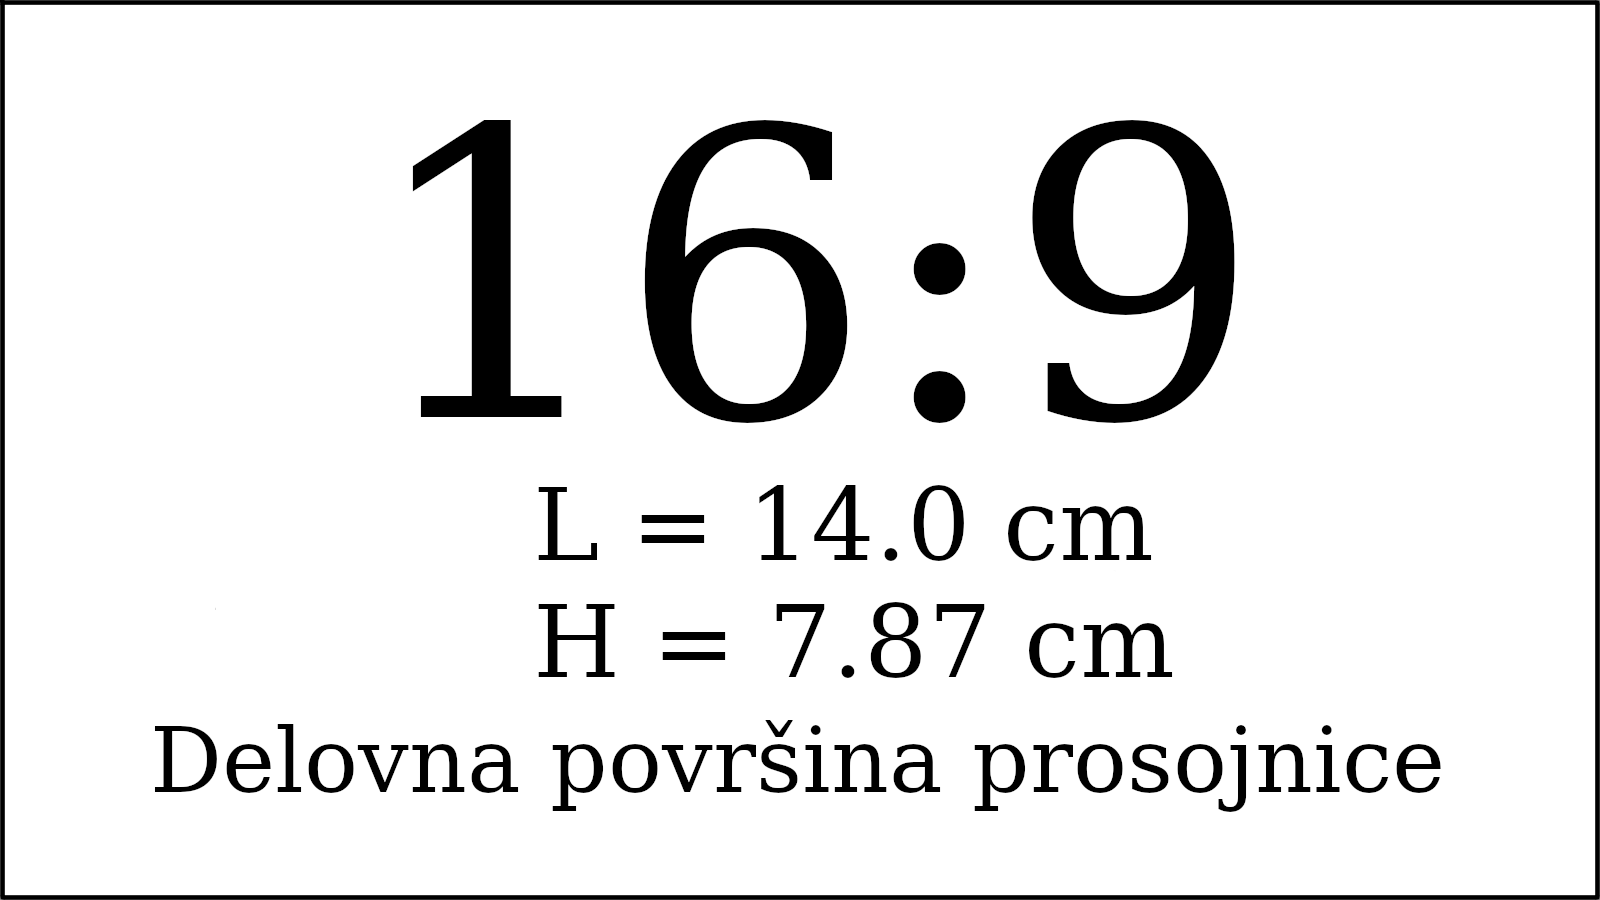
\includegraphics[width=13.9cm,height=7.8cm]{figs/169_frame.png} % višina + dolžina
	\end{center}	
	
\end{frame}

% *******************

\begin{frame}
	\frametitle{Uvod 1 - slika}
	
	Slikovna razlaga matrike kot tabele
	
	\vspace*{5mm}
	\begin{minipage}{7cm}
		\begin{center}
			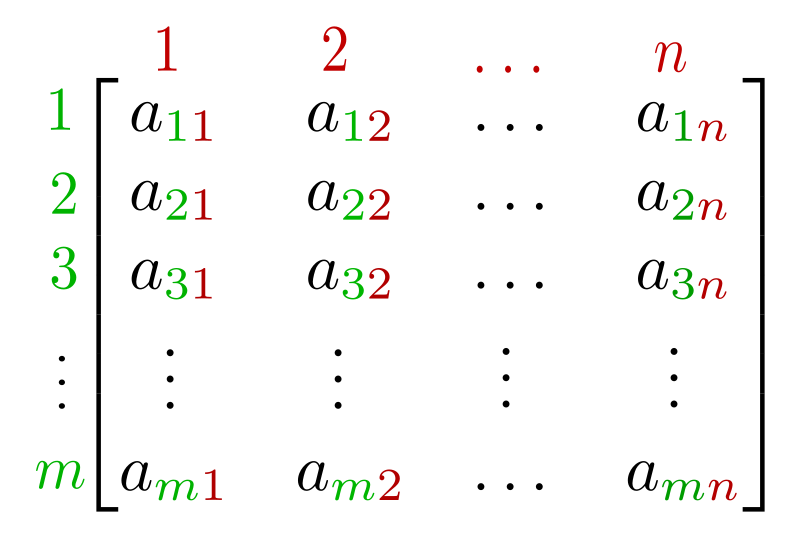
\includegraphics[height=4cm]{figs/matrix_01.png}
		\end{center}	
	\end{minipage}
	\hfill
	\begin{minipage}{7cm}
		\begin{center}
			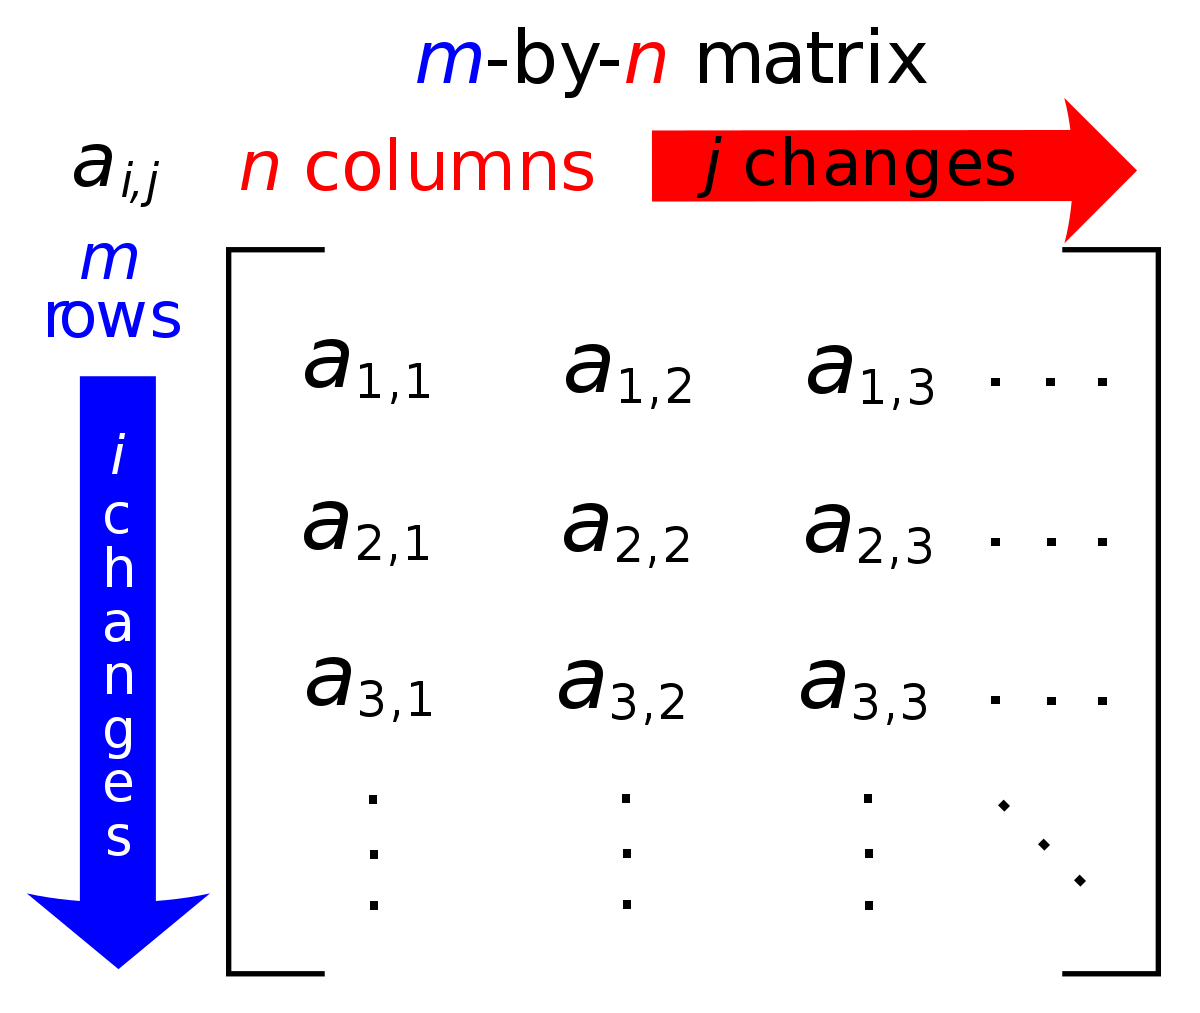
\includegraphics[height=4cm]{figs/matrix_02.png}
		\end{center}	
	\end{minipage}

\end{frame}

% *******************

\begin{frame}[fragile]
	\frametitle{Code insert}

	\lstinputlisting[language=Octave,style=mystyle]{figs/test.m}

\end{frame}

% ***************************
% ***** New Sub-Section *****
% ***************************
\subsection{Naslov pod poglavja}

% *** Sub-Section Frame ***
\begin{frame}[plain,noframenumbering,label=newsubsection]
	\vfill
	\begin{center}
		\textbf{\insertsubsectionhead}
	\end{center}
	\vfill
\end{frame}

% *******************

\begin{frame}
	\frametitle{Uvod 2}
	
	\emphc{Problem:} Poišči presečiščno točko treh ravnin, če je enačba ravnine zapisana z enačbo
	
	\[
	\alpha x + \beta y + \gamma z = p.
	\]
	
	\emphc{Primer:} Imamo sistem treh ravnin
	
	\begin{equation} \label{eq:plane_system}
		\begin{split}
			4 x + 2 y + z & = 7\\
			2 x + y - z & = 5\\
			x + 2 y + 2 z & = 3
		\end{split}	
	\end{equation}
	
	kjer je potrebno poiskati skupno točko $T(x,y,z)$.
\end{frame}

% *******************

\begin{frame}
	\frametitle{Uvod 3}
	
	\emphc{Problem:} Poišči presečiščno točko treh ravnin, če je enačba ravnine zapisana z enačbo
	
	\[
	\alpha x + \beta y + \gamma z = p.
	\]
	
	\emphc{Primer:} Imamo sistem treh ravnin
	
	\begin{equation} \label{eq:plane_system}
		\begin{split}
			4 x + 2 y + z & = 7\\
			2 x + y - z & = 5\\
			x + 2 y + 2 z & = 3
		\end{split}	
	\end{equation}
	
	kjer je potrebno poiskati skupno točko $T(x,y,z)$.
\end{frame}


% =======================
% ===== New Section =====
% =======================

\section{Matrike -- Ponovno}

% *** Section Frame ***
\begin{frame}[plain,noframenumbering,label=newsection]
	\vfill
	\begin{center}
		\boxed{\textcolor{royalblue1}{\textbf{Poglavje -- \thesection}}}
		
		\vspace*{5mm}
		\textcolor{royalblue1}{\textbf{\insertsectionhead}}
		%\textcolor{royalblue1}{\textbf{\insertsubsectionhead}}
	\end{center}
	\vfill
\end{frame}

% ===================

\begin{frame}
	\frametitle{Uvod 1}
	
	\emphc{Problem:} Poišči \emph{presečiščno} točko treh ravnin, če je \emph{enačba} ravnine zapisana z enačbo
	
	\[
	\alpha x + \beta y + \gamma z = p.
	\]
	
	\emphc{Primer:} Imamo sistem treh ravnin
	
	\begin{equation} \label{eq:plane_system}
		\begin{split}
			4 x + 2 y + z & = 7\\
			2 x + y - z & = 5\\
			x + 2 y + 2 z & = 3
		\end{split}	
	\end{equation}
	
	kjer je potrebno poiskati skupno točko $T(x,y,z)$.
	
\end{frame}

% *******************

\begin{frame}
	\frametitle{Prikaz delovne površine prosojnice \& največja velikost slike}
	
	%
	% Največja slikovna površina pri 16:9 formatu je:
	%  - širina L = 14.0 cm
	%  - višina H = 7.87 cm
	%
	% kot kaže spodnja slika.
	
	\begin{center}
		% Določanje velikosti slike:
		% - ohranimo "aspect ratio"
		%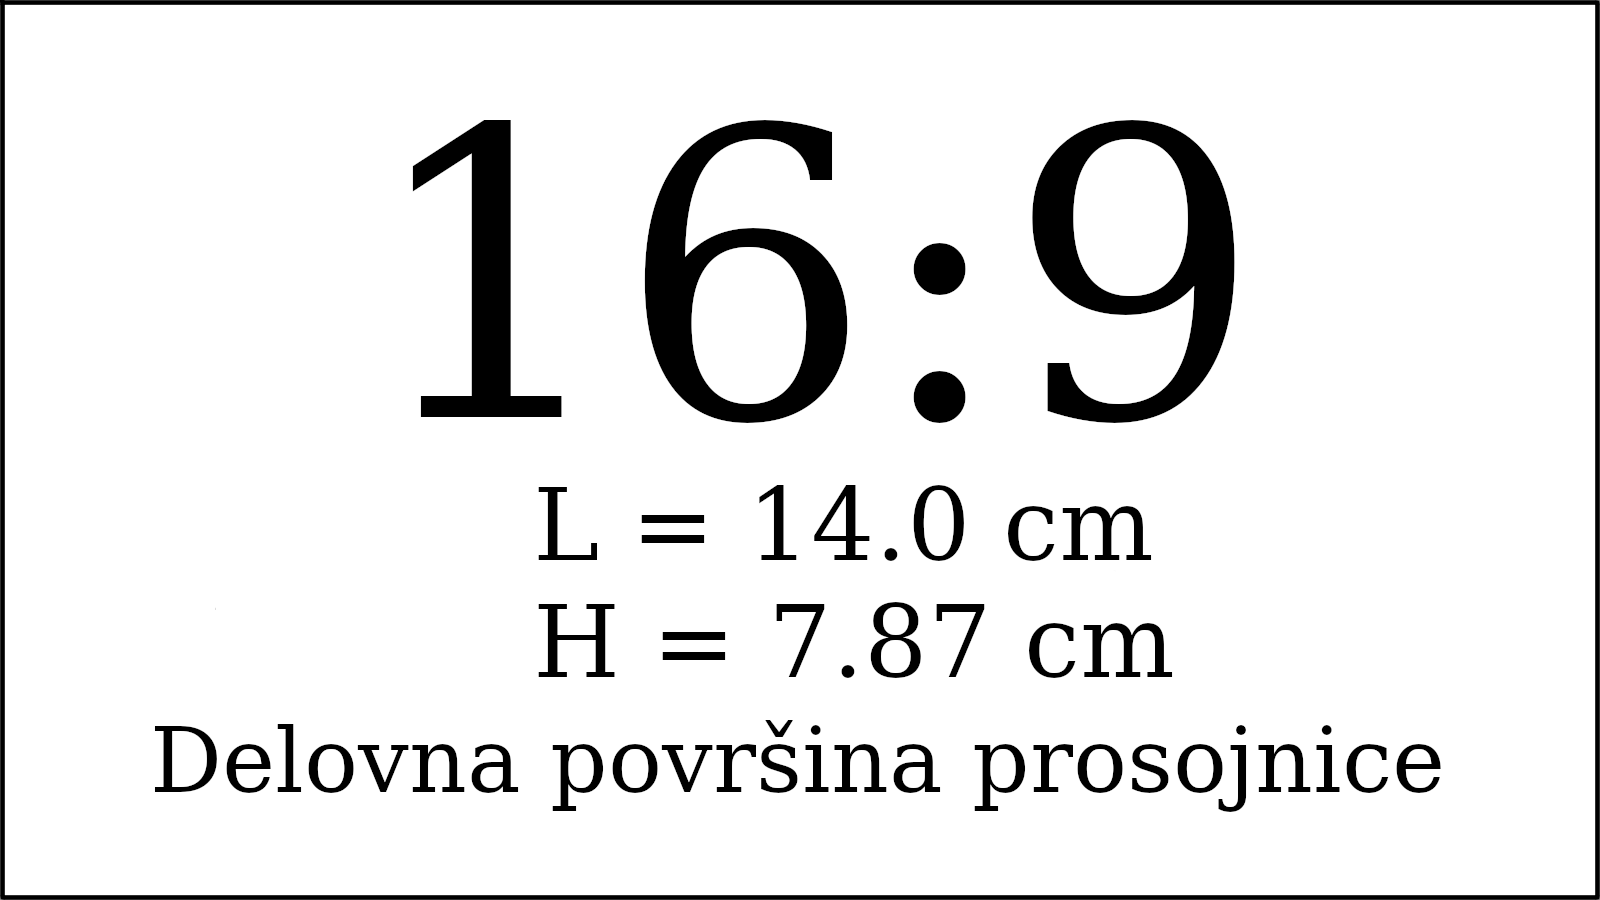
\includegraphics[width=13.9cm]{figs/169_frame.png} % dolžina
		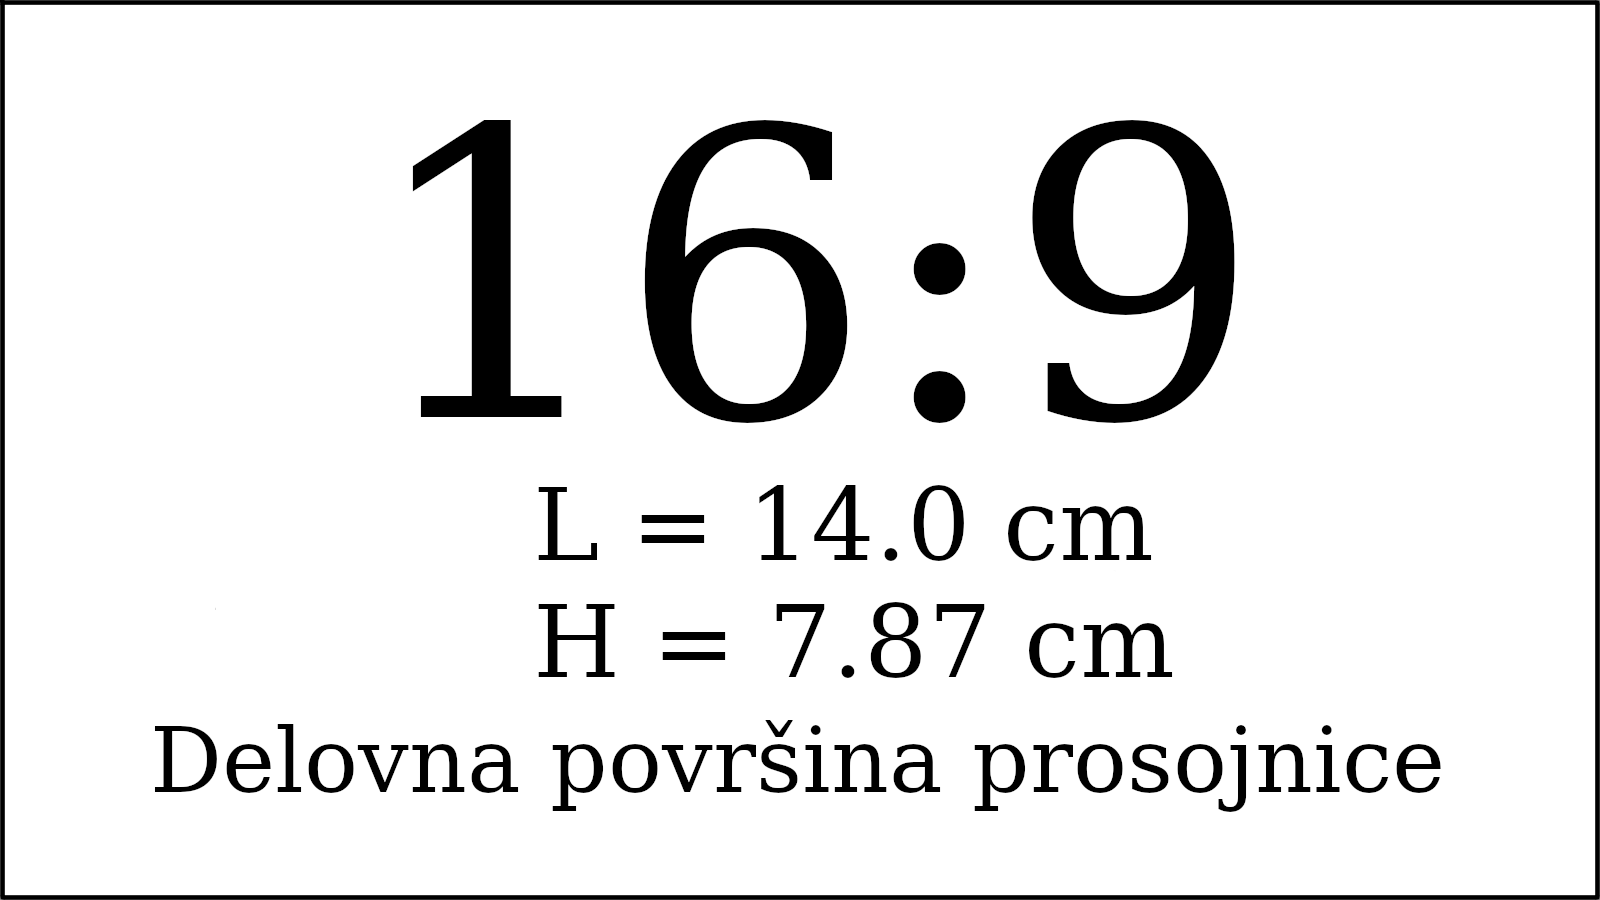
\includegraphics[height=7.7cm]{figs/169_frame.png} % višina
		%
		% - pokvarimo "aspect ratio"
		%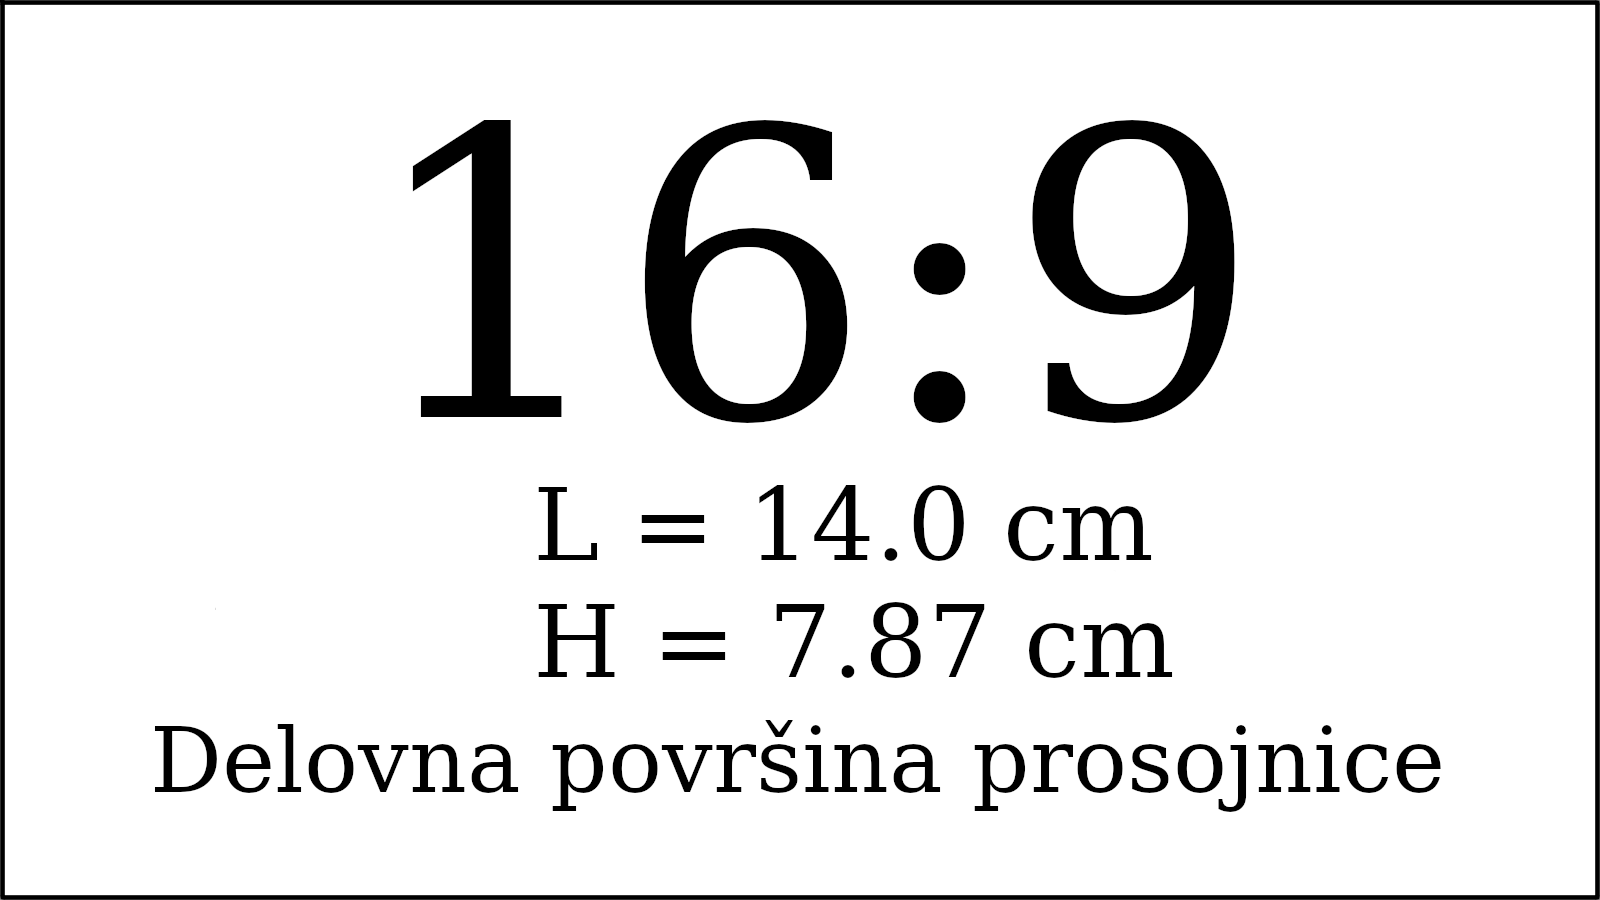
\includegraphics[width=13.9cm,height=7.8cm]{figs/169_frame.png} % višina + dolžina
	\end{center}	
	
\end{frame}

% ======================
% ===== References =====
% ======================

\section*{Literatura}

\begin{frame}[plain,noframenumbering,label=references]
	\vfill
	\begin{center}
		\textcolor{royalblue1}{\textbf{\Large Literatura}}
	\end{center}
	\vfill
\end{frame}

% ======================
	
\begin{frame}[plain]
	\frametitle{Literatura}
	\begin{itemize}
		\item G.~James, \emph{Modern Engineering Mathematics}, 2015, 5th Edition
		\item A.~Turnšek, \emph{Tehniška matematika}, 2007, 2.izdaja
	\end{itemize}
\end{frame}

\end{document} 
